\section{Nest Watcher}\label{sec:nest-watcher}
Tato služba interpretuje stavy jednotlivých hnízd v kurníku pro Home Assistanta.
Úkolem této služby je načítání a analýza dat z jednotlivých hnízd v kurníku.
Každé hnízdo je reprezentováno jednou instancí služby Scale Driver.\newline
V aktuální situaci služba obsluhuje šest hnízd, přičemž se data z každého hnízda monitorují a vyhodnocují.
Toto komplexní sledování umožňuje efektivní řízení kurníku, zajišťuje optimální péči o slepice a včasný sběr vajec.
Přístup založený na datech zvyšuje naši schopnost udržovat zdravé slepice a maximalizovat jejich produktivitu.\newline

\subsection*{Popis algoritmu}

Data jsou načítána několikrát za minutu a ukládána do databáze s časovým údajem, kdy byl záznam vytvořen.
Záznam v databázi obsahuje následující sloupce:

\begin{itemize}
    \item id - jednoznačný identifikátor záznamu v databáz.
    \item nest\_id - dentifikační číslo hnízda
    \item weight - naměřená hmotnost v gramech pro dané hnízdo
    \item timestamp - čas vytvoření záznamu
\end{itemize}

Následně se jednou za minutu vyhodnotí průměrná hodnota během posledních několika vážení.
Na základě vyhodnocené průměrné hmotnosti jsme schopni zjistit několik hlavních stavů hnízda:

\begin{itemize}
    \item Hnízdo je prázdné - pokud průměrná hmotnost nepřevyšuje 50 gramů (vzhledem k možným chybám měření), vyhodnotíme, že hnízdo je prázdné.
    V hnízdě není ani slepice, ani vejce.
    \item V hnízdě se nacházejí vejce - jestliže se hodnota hmotnosti pohybuje mezi 50 a 1200 gramy, znamená to, že v hnízdě jsou pravděpodobně vejce.
    Hmotnost jednoho vejce je přibližně 50 gramů, takže počet vajec lze vypočítat vydělením celkové hmotnosti hmotností jednoho vejce.
    \item V hnízdě sedí slepice - pokud je průměrná hmotnost na váze více než 1200 gramů, vyhodnotí služba, že v hnízdě sedí slepice.
    Hmotnost slepice se pohybuje kolem 1200 gramů a více.
\end{itemize}

Pro lepší pochopení jsem přiložil grafickou reprezentaci dat z databáze~(\ref{fig:weight_egg_chart_timeline}).
Znázorňuje vývoj hodnoty hmotnosti v čase pro konkrétní hnízdo.
Na ose x je znázorněn čas a na ose y je hmotnost.
Z grafu je možné odvodit následující příběh.
Ve dvacaté minutě vlezla slepice s hmotnosti kolem 2000 gramu na váhu.
Po 28 minutach ji opustila a zůstalo po ní snesené vejce s hmotnosti 55 gramu.
Další slepice vstoupila do hnízda ve 186 minutě a opustila hnizdo za 37 minut.
Následně pak váha ukazuje hmotnost kolem 115 gramu, což při znalosti hmotnosti jednoho vejce indikuje přítomnost 2 vajec.


\begin{figure}[H]
    \centering
    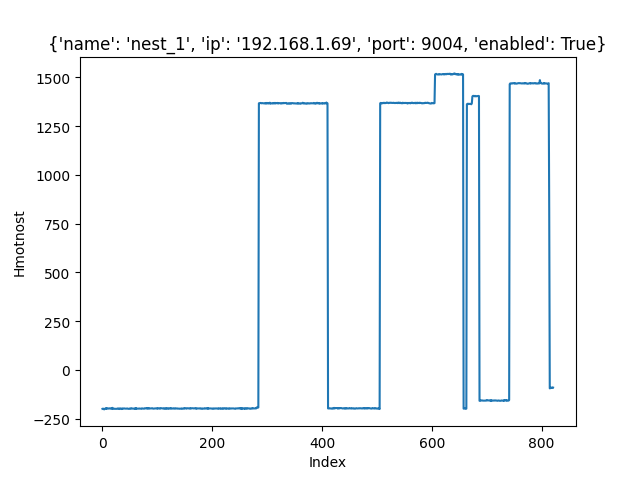
\includegraphics[width=0.8\textwidth]{img/weight_egg_chart_timeline}
    \captionAuthorSource{Graf vývoje hmotnosti hnízda v čase}
    \label{fig:weight_egg_chart_timeline}
\end{figure}

Výsledná data pro jednotlivá hnízda služba pomocí MQTT protokolu předává do systému Home Assistant, aby je zpracoval a vizualizoval chovateli.\newline


\subsection*{Popis možných vylepšení práce s váhou}
Díky měřením hmotnosti můžeme odvodit i další vzorce, které mohou být využity k diagnostice závady na váze a nebo identifikaci toho, že některá ze slepic má nějaký problém.
V případě, kdy by se data z váhy na základě času spojila společně se záběrem z kamery, dalo by se v tomto případě přesně určit, o kterou ze slepic se jedná. \newline
Určit by slepice mohl jednak chovatel díky tomu, že by mu byl předložen snímek, na němž je slepice v konkrétním hnízdě, které hlásí problém.
Konkrétní slepici by časem mohla detekovat i neuronová síť. \newline
Toto řešení je však velmi komplikované, protože vzhledem k vysoké podobnosti bude složité rozlišit například dvě podobně bílé slepice a chovateli jednoznačně sdělit, která slepice má problém.
Na druhou stranu, pokud by se tento princip reidentifikace dovedl k dokonalosti, přinesl by revoluci monitoringu pomocí kamerových systémů.
Dále se o implementaci vlastního reidentifikačního algoritmu hovoří v sekci~\ref{sec:koncept-identifikace-nejlepsi-nosnice}.
\newline
Kromě výše zmíněných stavů by se v budoucnu z váhy dal identifikovat i následující seznam situací.

\begin{itemize}
    \item Doba setrvání slepice v hnízdě - analýzou délky období, kdy je hmotnost hnízda nad 1200 gramů, lze zjistit, jak dlouho slepice v hnízdě zůstává.
    To může upozornit na možné zdravotní problémy, pokud setrvává v hnízdě déle než obvykle.
    \item Frekvence snášení u jednotlivých hnízd - porovnáním počtu snesených vajec v různých hnízdech lze zjistit, zda některá hnízda nejsou preferována více než jiná.
    To může vést k úpravám uspořádání kurníku nebo kontrolám hnízd, která jsou méně využívána.
    \item Poruchy senzorů - pokud hmotnost zůstává nezměněna po dlouhou dobu nebo vykazuje nerealistické hodnoty, může to indikovat technickou závadu.
    Pravidelná kontrola a kalibrace senzorů zajistí spolehlivost dat.
    \item Denní vzorce aktivity - analýzou hmotnostních dat během dne lze určit období nejvyšší aktivity slepic.
    To může být užitečné pro plánování krmení, čištění kurníku nebo jiných činností, které by mohly slepice rušit.
\end{itemize}

%\subsection*{Předpokládaná datová struktura v databázi:}
%
%\begin{table}[h!]
%    \centering
%    \begin{tabular}{lll}
%        \textbf{Pole} & \textbf{Datový typ} & \textbf{Popis}                                    \\
%        timestamp     & DATETIME            & Datum a čas měření                                \\
%        nid           & INT                 & Identifikační číslo hnízda (1 až 6)               \\
%        weight        & FLOAT               & Naměřená hmotnost v gramech                       \\
%        nest\_status  & VARCHAR             & Stav hnízda (např. "prázdné", "vejce", "slepice") \\
%    \end{tabular}
%    \captionAuthorSource{Datová struktura v databázi}
%\end{table}
%
%Tato datová struktura umožňuje efektivní ukládání a vyhodnocování dat z jednotlivých hnízd. Pole \texttt{nest\_status} může být automaticky vypočítáno na základě hodnoty v poli \texttt{weight} podle výše uvedených kritérií. Tímto způsobem můžeme snadno filtrovat a analyzovat data pro sledování stavu každého hnízda v čase.
%
%Rozšířená analýza nám poskytuje hlubší vhled do chování slepic a umožňuje nám přijímat informovaná rozhodnutí pro zlepšení podmínek v kurníku, zvýšení produktivity a zajištění pohody zvířat.

%Data jsou načítána několikrát do minuty a ukládána do databáze s časovým údajem, kdy byl záznam vytvořen.
%Následně se jednou za minutu vyhodnotí průměrná hodnota během posledních několika vážení.
%Na základě tohoto údaje jsme schopni zjisti několik případů
%\begin{itemize}
%    \item hnízdo je prázdné (hodnota na váze nepřevyšuje 50 g )
%    \item v hnízdě se nacházejí vejce (hmotnost jednoho vejce je průměrně 50 g)
%    \item v hnízdě sedí slepice (hmotnost slepice se pohybuje okolo 1200 g a více)
%\end{itemize}
%Pokud je na váze průměrně méně než 50 g, vzhledem k možným chybám měření, takový případ vyhodnotíme jako, že je hnízdo prázdné.
%Jestliže se hodnota pohybuje mezi 50 a 1200 gramy, znamená to, že v hnízdě jsou pravděpodobně vejce, a jejich počet je vypočítán vydělením celkové hmotnosti a hmotnosti jednoho vejce.
%V případě, že je na váze více jak 1200 g, vyhodnotí služba, že v hnízdě sedí slepice.
%Tyto tři zmíněné informace služba následně pomocí MQTT předává do Home Assistanta.
